\documentclass[CJK]{beamer}
%\usepackage{CJKutf8}
\usepackage{beamerthemesplit}
\usepackage{}
%\usetheme{Frankfurt}
%\usetheme{CambridgeUS}
%\usecolortheme{beaver}
%\usetheme{AnnArbor}
\usetheme{Dresden}
%\usebeamercolor{beetle}
\usepackage{xeCJK}
\setCJKmainfont{AR PL KaitiM GB}
%\useoutertheme{miniframes}
\usepackage{amsmath}
\usepackage{graphicx}
\usepackage{float} 
\usepackage{subfigure}
\usepackage{amssymb}
\usepackage{graphicx}
\usepackage{eufrak}
\usepackage{color}
\usepackage{array}
\usepackage{slashed}
\usepackage{simplewick}
\usepackage{tikz}
\usepackage{tcolorbox}
\usepackage[T1]{fontenc}
\graphicspath{{../figures/}}

%%figures
\def\lfig#1#2{\includegraphics[width=#1 in]{#2}}
\def\addfig#1#2{\begin{center}\includegraphics[width=#1 in]{#2}\end{center}}
\def\wulian{
\includegraphics[width=0.18in]{emoji_wulian.jpg}}
\def\bigwulian{
\includegraphics[width=0.35in]{emoji_wulian.jpg}}
\def\bye{
\includegraphics[width=0.18in]{emoji_bye.jpg}}
\def\bigbye{
\includegraphics[width=0.35in]{emoji_bye.jpg}}
\def\huaixiao{
\includegraphics[width=0.18in]{emoji_huaixiao.jpg}}
\def\bighuaixiao{
\includegraphics[width=0.35in]{emoji_huaixiao.jpg}}
\def\jianxiao{
\includegraphics[width=0.18in]{emoji_jianxiao.jpg}}
\def\bigjianxiao{
\includegraphics[width=0.35in]{emoji_jianxiao.jpg}}
%% colors
\def\blacktext#1{{\color{black}#1}}
\def\bluetext#1{{\color{blue}#1}}
\def\redtext#1{{\color{red}#1}}
\def\darkbluetext#1{{\color[rgb]{0,0.2,0.6}#1}}
\def\skybluetext#1{{\color[rgb]{0.2,0.7,1.}#1}}
\def\cyantext#1{{\color[rgb]{0.,0.5,0.5}#1}}
\def\greentext#1{{\color[rgb]{0,0.7,0.1}#1}}
\def\darkgray{\color[rgb]{0.2,0.2,0.2}}
\def\lightgray{\color[rgb]{0.6,0.6,0.6}}
\def\gray{\color[rgb]{0.4,0.4,0.4}}
\def\blue{\color{blue}}
\def\red{\color{red}}
\def\green{\color{green}}
\def\darkgreen{\color[rgb]{0,0.4,0.1}}
\def\darkblue{\color[rgb]{0,0.2,0.6}}
\def\skyblue{\color[rgb]{0.2,0.7,1.}}
%%control
\def\be{\begin{equation}}
\def\ee{\nonumber\end{equation}}
\def\bea{\begin{eqnarray*}}
\def\eea{\nonumber\end{eqnarray*}}
\def\bch{}
\def\ech{}
\def\bitem{\begin{itemize}}
\def\eitem{\end{itemize}}
\def\bcenter{\begin{center}}
\def\ecenter{\end{center}}
\def\bex{\begin{minipage}{0.2\textwidth}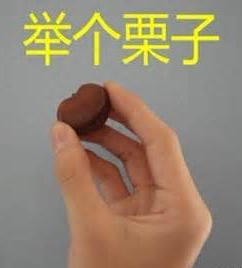
\includegraphics[width=0.6in]{jugelizi.png}\end{minipage}\begin{minipage}{0.76\textwidth}}
\def\eex{\end{minipage}}
\def\chtitle#1{\frametitle{\bch#1\ech}}
\def\bmat#1{\left(\begin{array}{#1}}
\def\emat{\end{array}\right)}
\def\bcase#1{\left\{\begin{array}{#1}}
\def\ecase{\end{array}\right.}
\def\bmini#1{\begin{minipage}{#1\textwidth}}
\def\emini{\end{minipage}}
\def\tbox#1{\begin{tcolorbox}#1\end{tcolorbox}}
\def\pfrac#1#2#3{\left(\frac{\partial #1}{\partial #2}\right)_{#3}}
%%symbols
\def\bropt{\,(\ \ \ )}
\def\sone{$\star$}
\def\stwo{$\star\star$}
\def\sthree{$\star\star\star$}
\def\sfour{$\star\star\star\star$}
\def\sfive{$\star\star\star\star\star$}
\def\rint{{\int_\leftrightarrow}}
\def\roint{{\oint_\leftrightarrow}}
\def\stdHf{{\textit{\r H}_f}}
\def\deltaH{{\Delta \textit{\r H}}}
\def\ii{{\dot{\imath}}}
\def\skipline{{\vskip0.1in}}
\def\skiplines{{\vskip0.2in}}
\def\lagr{{\mathcal{L}}}
\def\hamil{{\mathcal{H}}}
\def\vecv{{\mathbf{v}}}
\def\vecx{{\mathbf{x}}}
\def\vecy{{\mathbf{y}}}
\def\veck{{\mathbf{k}}}
\def\vecp{{\mathbf{p}}}
\def\vecn{{\mathbf{n}}}
\def\vecA{{\mathbf{A}}}
\def\vecP{{\mathbf{P}}}
\def\vecsigma{{\mathbf{\sigma}}}
\def\hatJn{{\hat{J_\vecn}}}
\def\hatJx{{\hat{J_x}}}
\def\hatJy{{\hat{J_y}}}
\def\hatJz{{\hat{J_z}}}
\def\hatj#1{\hat{J_{#1}}}
\def\hatphi{{\hat{\phi}}}
\def\hatq{{\hat{q}}}
\def\hatpi{{\hat{\pi}}}
\def\vel{\upsilon}
\def\Dint{{\mathcal{D}}}
\def\adag{{\hat{a}^\dagger}}
\def\bdag{{\hat{b}^\dagger}}
\def\cdag{{\hat{c}^\dagger}}
\def\ddag{{\hat{d}^\dagger}}
\def\hata{{\hat{a}}}
\def\hatb{{\hat{b}}}
\def\hatc{{\hat{c}}}
\def\hatd{{\hat{d}}}
\def\hatN{{\hat{N}}}
\def\hatH{{\hat{H}}}
\def\hatp{{\hat{p}}}
\def\Fup{{F^{\mu\nu}}}
\def\Fdown{{F_{\mu\nu}}}
\def\newl{\nonumber \\}
\def\vece{\mathrm{e}}
\def\calM{{\mathcal{M}}}
\def\calT{{\mathcal{T}}}
\def\calR{{\mathcal{R}}}
\def\barpsi{\bar{\psi}}
\def\baru{\bar{u}}
\def\barv{\bar{\upsilon}}
\def\qeq{\stackrel{?}{=}}
\def\torder#1{\mathcal{T}\left(#1\right)}
\def\rorder#1{\mathcal{R}\left(#1\right)}
\def\contr#1#2{\contraction{}{#1}{}{#2}#1#2}
\def\trof#1{\mathrm{Tr}\left(#1\right)}
\def\trace{\mathrm{Tr}}
\def\comm#1{\ \ \ \left(\mathrm{used}\ #1\right)}
\def\tcomm#1{\ \ \ (\text{#1})}
\def\slp{\slashed{p}}
\def\slk{\slashed{k}}
\def\calp{{\mathfrak{p}}}
\def\veccalp{\mathbf{\mathfrak{p}}}
\def\Tthree{T_{\tiny \textcircled{3}}}
\def\pthree{p_{\tiny \textcircled{3}}}
\def\dbar{{\,\mathchar'26\mkern-12mu d}}
\def\erf{\mathrm{erf}}
\def\const{\mathrm{constant}}
\def\pheat{\pfrac p{\ln T}V}
\def\vheat{\pfrac V{\ln T}p}
%%units
\def\fdeg{{^\circ \mathrm{F}}}
\def\cdeg{^\circ \mathrm{C}}
\def\atm{\,\mathrm{atm}}
\def\angstrom{\,\text{\AA}}
\def\SIL{\,\mathrm{L}}
\def\SIkm{\,\mathrm{km}}
\def\SIyr{\,\mathrm{yr}}
\def\SIGyr{\,\mathrm{Gyr}}
\def\SIV{\,\mathrm{V}}
\def\SImV{\,\mathrm{mV}}
\def\SIeV{\,\mathrm{eV}}
\def\SIkeV{\,\mathrm{keV}}
\def\SIMeV{\,\mathrm{MeV}}
\def\SIGeV{\,\mathrm{GeV}}
\def\SIcal{\,\mathrm{cal}}
\def\SIkcal{\,\mathrm{kcal}}
\def\SImol{\,\mathrm{mol}}
\def\SIN{\,\mathrm{N}}
\def\SIHz{\,\mathrm{Hz}}
\def\SIm{\,\mathrm{m}}
\def\SIcm{\,\mathrm{cm}}
\def\SIfm{\,\mathrm{fm}}
\def\SImm{\,\mathrm{mm}}
\def\SInm{\,\mathrm{nm}}
\def\SImum{\,\mathrm{\mu m}}
\def\SIJ{\,\mathrm{J}}
\def\SIW{\,\mathrm{W}}
\def\SIkJ{\,\mathrm{kJ}}
\def\SIs{\,\mathrm{s}}
\def\SIkg{\,\mathrm{kg}}
\def\SIg{\,\mathrm{g}}
\def\SIK{\,\mathrm{K}}
\def\SImmHg{\,\mathrm{mmHg}}
\def\SIPa{\,\mathrm{Pa}}
\def\secpage#1#2{\begin{frame}\bch\bcenter{\bf \Huge #1} \skipline \tbox{\bcenter #2\ecenter}\ecenter\ech\end{frame}}



\newcommand{\field}{\mathscr{F}}

\newcommand{\reals}{\mathbb{R}}
\newcommand{\complexs}{\mathbb{C}}
\newcommand{\ints}{\mathbb{Z}}
%\newcommand{\dim}{\mathrm{dim\ }}
\newcommand{\diag}{\mathrm{diag \ }}
\newcommand{\up}{\uparrow}
\newcommand{\down}{\downarrow}
\newcommand{\su}{\mathfrak{su}}
\newcommand{\so}{\mathfrak{so}}
\newcommand{\tr}{\mathrm{tr\ }}
\newcommand{\card}{\mathrm{card \ }}

\newtheorem{thm}{定理}[section]
\newtheorem{axm}{公理}[section]
\newtheorem{dfn}{定义}[section]

%\cpic{<尺寸>}{<文件名>}}用于生成居中的图片。
\newcommand{\cpic}[2]{
\begin{center}
\includegraphics[scale=#1]{#2}
\end{center}
}

%\cpicn{<尺寸>}{<文件名>}{<注释>}用于生成居中且带有注释的图片,其label为图片名。
\newcommand{\cpicn}[3]
{
\begin{figure}[h!]
\cpic{#1}{#2}
\caption{#3\label{#2}}
\end{figure}
}

\title{Group Theory\\ The Eightfold way of $SU(3)$}
  \author{Haoting Xu}
  \date{2019.11}


\begin{document}

\begin{frame}
 
\begin{center}
\begin{Large}
\bch
{\bf G}roup {\bf T}heory

{\vskip 0.3in}

The Eightfold way of $SU(3)$

\ech
\end{Large}
\end{center}

\vskip 0.2in
\begin{center}
Haoting Xu
\vskip 0.1in
xuht9@mail2.sysu.edu.cn
\vskip 0.2in
{\tiny \url{https://github.com/HaotingXu/seminar_lec} }\\
\end{center}
\end{frame}

\section{Introduction}
\secpage{Introduction}{吹水}
\begin{frame}\frametitle{S.L Glashow's fortune}
  \bch
  While most of our colleagues were put off by the unfamiliar
math, [Sidney Coleman and I] became traveling disciples of the
Eightfold Way.

- Sheldon Lee Glashow(received the Nobel Prize in 1979 for work based to a large extent on
group theory.)
\cpicn{0.15}{glashow}{Sheldon Lee Glashow}
\ech
\end{frame}

\begin{frame}
  \bch
  仰天大笑吧!困惑上世纪六十年代顶尖粒子物理学家的数学不过只是$SU(3)$!五分钟就能学完。
  \cpic{0.3}{az}
  \ech
\end{frame}
\begin{frame}\frametitle{\bch 粒子物理中的$SU(3)$\ech}
  \bch
  我们已经见过了$SU(2)$的威力,它贯穿整个量子力学,它也在经典物理中出现。$SU(3)$只在粒子物理中出现,而且出现了两次
  \begin{itemize}
  \item 夸克的发现
  \item 量子色动力学的规范对称群
  \end{itemize}
  \ech
\end{frame}

\section{Tensors}
\secpage{使用张量方法构造表示}{$D(m,n)=\frac{1}{2}(m+1)(n+1)(m+n+2)$}
\begin{frame}\frametitle{\bch 张量方法构造表示\ech}
  \bch
  我们还是用张量的方法构造表示,回忆$SU(N)$群中要区分上下标,比如对于$SU(2)$群,有
  \be
  \psi_i = \epsilon_{ij}\psi^j
  \ee
  因此,我们说上标和下标实际上可以不做区分,是等价的。但是对于$SU(3)$群,显然上标和下标不等价,尝试这样缩并只会得到更高阶的张量。
  \ech
\end{frame}
\begin{frame}\frametitle{\bch 上标和下标\ech}
  \bch
  因此,我们需要单独处理上标和下标,我们记有$m$个上标和$n$个下标的张量为$(m,n)$型张量。虽然$SU(3)$需要区分上下标,但是它仍然有非常好的性质,我们将证明,只需要考虑无迹且上下标分别对称的张量。证明如下
  \begin{itemize}
  \item 取一个$(m,n)$型张量,取定两个指标,构造他们的对称部分、反对称部分和迹,将无迹对称张量纳入考虑。用特殊方法抽掉的迹也是对称张量。
  \item 将反对称部分使用$\epsilon_{ijk}$缩并,就会将两个反对称上(下)指标变成一个下(上)指标,如此往复操作(再进行对称反对称、抽迹),直到剩余$(1,1)$型张量。
  \item 这样剩余的全部是我们要的张量,证毕。
  \end{itemize}
  \ech
\end{frame}
\begin{frame}\frametitle{小练习}
  \bch
  试构造$T^{ij}_{kl}$的无迹对称部分
  \be
  \tilde{T}^{ij}_{kl} = T^{ij}_{kl} - A(\delta^i_kT^j_l+\delta^j_kT^i_l+\delta^i_lT^j_k+\delta^j_lT^i_k)+B(\delta^i_k\delta^j_l+\delta^j_k\delta^i_l+\delta^i_l\delta^j_k+\delta^j_l\delta^i_k)T
  \ee
  其中$T^j_l = T^{ij}_{il}$,$T = T^j_j$
  \ech
\end{frame}

\begin{frame}\frametitle{\bch$SU(3)$表示的维数\ech}
  \bch
  因此,全体$(m,n)$型无迹对称张量得到的表示就是$SU(3)$用这种方法得到的所有不可约表示。我们下面研究表示的维数。表示的维数就是张量的独立分量数,先只考虑对称。注意到$i,j,k$等指标在$SU(3)$群里只能取$1,2,3$。假设有一个$(m,0)$张量$S^{33\cdots 3xx\cdots x}$,假设有$k$个指标不是$3$,即有$k$个$x$,在这种情况下,看$k$个$1,2$中有多少个$1$,故独立分量个数为
  \be
  \sum_{k=0}^{m}(k+1) = \frac{1}{2}(m+1)(m+2)
  \ee
  \ech
\end{frame}
\begin{frame}\frametitle{\bch$SU(3)$表示的维数 \ech}
  \bch
  因此,$(m,n)$型上下指标分别对称的张量的独立分量就有$\frac{1}{4}(m+1)(m+2)(n+1)(n+2)$个,现在考虑无迹的等式
  \be
  \delta^{j}_i \varphi^{ii_2\cdots i_m}_{jj_2\cdots j_m}=0
  \ee
  等式左边的行为像一个$(m-1,n-1)$型张量,所以一共有$\frac{1}{4}m(m+1)n(n+1)$个等式。因此,$(m,n)$型张量得到的表示维数为
  \bea
  D(m,n) &=& \frac{1}{4}(m+1)(m+2)(n+1)(n+2) - \frac{1}{4}m(m+1)n(n+1) \\
  &=& \frac{1}{2}(m+1)(n+1)(m+n+2)
  \eea
  \ech
\end{frame}
\begin{frame}\frametitle{\bch 一些例子\ech}
  \bch
  通过上面的公式计算一些特殊的例子,如下
  \cpic{0.3}{ex}
  \ech
\end{frame}
\begin{frame}\frametitle{\bch 将张量相乘\ech}
  \bch
  在$SU(2)$中,我们将两个张量乘起来得到一堆张量,这在代数中其实对应于角动量的加法。那么相应的,我们也来研究$SU(3)$的加法,以后我们会看到和$\su(3)$代数的联系。我们先算几个简单的例子。
  \ech
\end{frame}
\begin{frame}\frametitle{ 一些记号}
  \bch
  也可以用维数来表示张量。但是,$(1,0)$型张量和$(0,1)$型张量都贡献三维表示由于上下标不等价,所以应该做区分,前者记为$3$,后者记为$3^{*}$。同理,$(3,0)$型(无迹对称)张量得到的表示记作$10$,$(0,3)$型张量得到的表示记作$10^{*}$,以此类推。
  \ech
\end{frame}
\begin{frame}\frametitle{\bch 例1:$3\otimes 3^{*} = 8\oplus 1$\ech}
  \bch
  现在我们将张量直接“相乘”,我们先来计算$(1,0)\otimes (0,1)$,这意味着拼成一个张量$T^i_j$,根据套路,分成对称、反称(这里因为上标下标只有一个,所以没得构造)、迹三部分,迹是一个标量$(0,0)$,剩下的无迹部分便是一个$(1,1)$型表示。所以我们得到
  \be
  (1,0)\otimes(0,1) = (1,1)\oplus (0,0)
  \ee
  即
  \be
  3\otimes 3^{*} = 8\oplus 1
  \ee
  \ech
\end{frame}
\begin{frame}\frametitle{\bch 例2:$3\otimes 3 = 6\oplus 3^{*}$ \ech}
  \bch
  我们来计算$(1,0)\otimes (1,0)$,首先他们拼成一个$(2,0)$型张量,$(2,0)$型张量没的抽迹。将它拆成对称部分和反称部分,对称部分为$(2,0)$型对称张量,反对称部分利用$\chi_i = \epsilon_{ijk}A^{jk}$,这样将两个上标变成一个下标,得到一个$(0,1)$型张量。于是
  \be
  (1,0)\otimes (1,0) = (2,0)\oplus (0,1)
  \ee
  即
  \be
  3\otimes 3 = 6\oplus 3^{*}
  \ee
  \ech
\end{frame}

\begin{frame}\frametitle{\bch 例3:$3\otimes 6 = 10\oplus 8 $\ech}
  \bch
  再来算一个例子$(1,0)\otimes (2,0)$。他们先弄出一个$(3,0)$型张量,将$(3,0)$型张量分为对称部分、反称部分和迹。这里只有上指标,所以没有迹。利用$\epsilon$将两个上指标变成一个下指标,得到一个$(1,1)$型张量,就没得抽了。因此,我们得到
  \be
  (1,0)\otimes (2,0) = (3,0) \oplus (1,1)
  \ee
  即
  \be
  3\otimes 6 = 10\oplus 8
  \ee
  \ech
\end{frame}
\begin{frame}\frametitle{例4:$3\otimes 3\otimes 3$\ech}
  \bch
  利用上面三个例子得到的关系,得到
  \bea
  3\otimes 3\otimes 3 &=&  (6\oplus 3^{*})\otimes 3\\
  &=& (6\otimes 3)\oplus (3^{*}\otimes 3)\\
  &=& 10 \oplus 8\oplus 8\oplus 1\\
  \eea
  \ech
\end{frame}
\begin{frame}\frametitle{例5:$8\otimes 8$\ech}
  \bch
  大家自己做个练习
  \be
  (1,1)\otimes (1,1) = (2,2)\oplus (3,0)\oplus (0,3)\oplus (1,1)\oplus (1,1) \oplus (0,0)
  \ee
  \ech
\end{frame}  

\begin{frame}\frametitle{\bch 一般情况\ech}
  \bch
  有了上面的例子,我们现在可以来讨论一般情况,考虑$(m,n)\otimes (m^\prime,n^\prime)=(m,n;m^\prime,n^\prime)$,由于$(m,n)$和$(m^\prime,n^\prime)$已经是无迹对称的,所以抽取迹的操作应该对于不同张量的部分。例如,只能缩并$m$个上标中的一个指标和$n^\prime$下标中的一个。所以得到
  \bea
  (m,n)\otimes (m^\prime,n^\prime)&=& (m,n;m^\prime,n^\prime) \\
  &\oplus& (m-1,n;m^\prime,n^\prime-1)\oplus (m,n-1;m^\prime-1,n^\prime)\\
  &\oplus& (m-1,n-1;m^\prime-1,n^\prime-1)\\
  &\oplus& (m-2,n;m^\prime,n^\prime-2)\\
  &\oplus& \cdots ||
  \eea
  其中$||$表示当没有指标可以缩并的时候,这个过程终止。
  \ech
\end{frame}
\begin{frame}\frametitle{\bch 一般情况\ech}
  \bch
  最终,我们拿掉了所有的迹,得到$(m-p,n-q;m^\prime -q,n^\prime -p)$,注意这时候我们还没有关注张量是对称的还是反称的,接下来操作的一般表示就写不下去了,就举一个$8\otimes 8$的例子。

  $(1,1)\otimes (1,1)$进行疯狂抽迹操作,得到
  \be
  (1,1)\otimes (1,1) = (1,1;1,1) \oplus (0,1;1,0)\oplus (1,0;0,1)\oplus (0,0;0,0)
  \ee
  现在构造对称与反称张量,得到
  \be
  (1,1;1,1) = (2,2)\oplus (3,0)\oplus (0,3)
  \ee
  其它的都不用构造了,因为上标或者下标仅有一个指标。
  \ech
\end{frame}
\section{Particle Physics}
\secpage{$SU(3)$与粒子物理}{$SU(3)$基础表示是夸克}
\begin{frame}\frametitle{\bch 粒子物理的实验发现\ech}
  \bch
  在1950-1960,发现了一系列粒子。
  \begin{itemize}
  \item $\Lambda$重子在1950年被发现,质量1115$\mathrm{MeV}$,质量和中子、质子几乎相同,自旋与质子和中子一致。S.Sakata 推广了$SU(2)$同位旋到$SU(3)$中。
  \item 不幸的是,其他质量相近的重子被发现了:$\Sigma^{+},\Sigma^0,\Sigma^-$,质量约为$1190\mathrm{MeV}$,$\Xi^-,\Xi^0$,质量约为$1320\mathrm{MeV}$。到此,发现了八种重子$\Sigma^{+}$,$\Sigma^0$,$\Sigma^-$,$\Xi^-$,$\Xi^0$,$\Lambda$,$n$,$p$。
    \item 还新发现了四种赝无自旋的介子:$K^+,K^0,\bar{K}^0,K^-$(质量约为$495\mathrm{MeV}$),他们的性质像三个$\pi$介子(质量约为$138\mathrm{MeV}$)。故一共发现了七种介子$K^+,K^0,\bar{K}^0,K^-,\pi^+,\pi^-,\pi^0$。
  \end{itemize}
  \ech
\end{frame}
\begin{frame}\frametitle{The Particle Zoo}
  \bch
  感觉很乱?那就对了。
  \cpicn{0.25}{zoo}{The Particle Zoo}
  \ech
\end{frame}

\begin{frame}\frametitle{\bch $7$?\ech}
  \bch
  可见,发现了七种介子和八种重子。这时一些优秀的理论物理学家指出,$\Lambda,\Sigma^0$有不同的宇称,故应该把$\Lambda$除掉。一时之间,很多理论物理学家都在找有7维不可约表示的对称群。
  \ech
\end{frame}
\begin{frame}\frametitle{\bch The Eightfold Way\ech}
  \bch
  最终,另外一个赝无自旋的粒子$\eta$,被发现了。质量大约$550\mathrm{MeV}$。而且实验证实,$\Lambda,\Sigma^0$有相同的宇称。
  \begin{figure}
\centering  
\subfigure{
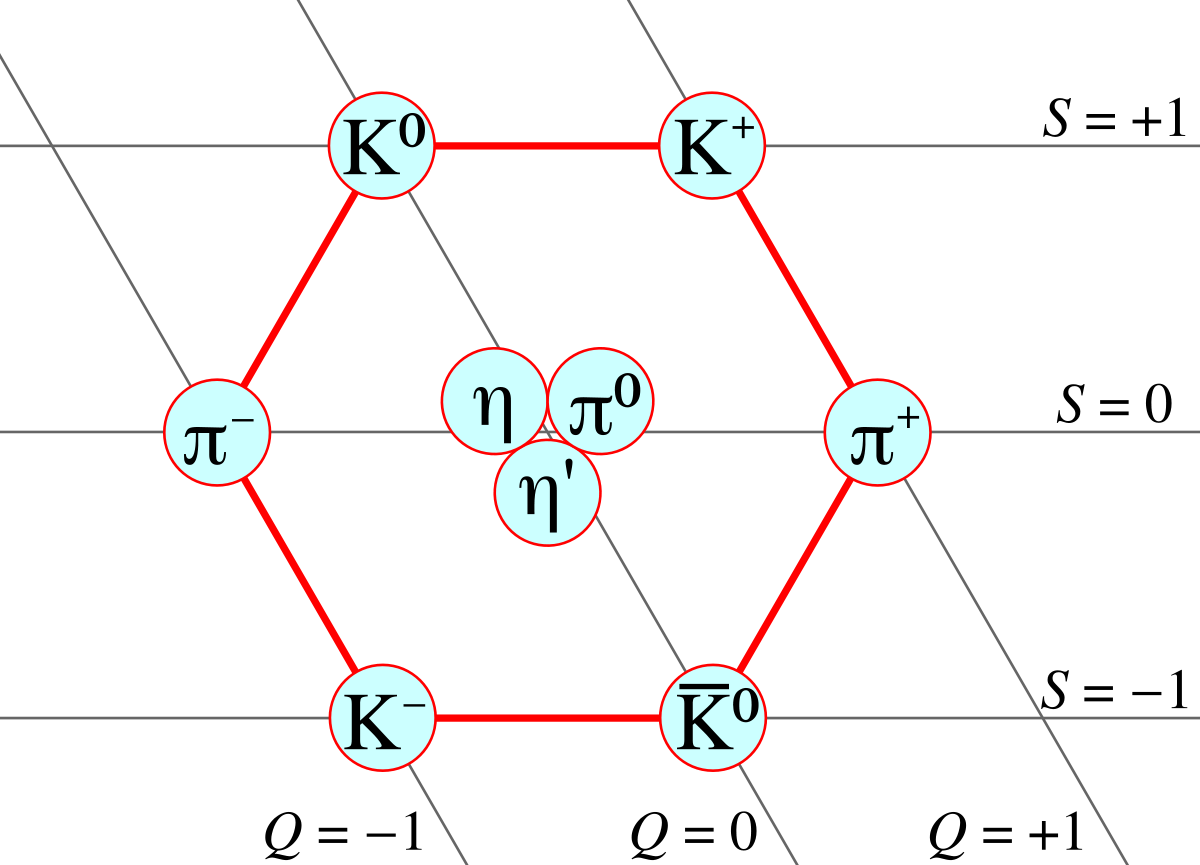
\includegraphics[width=0.45\textwidth]{meson}}
\subfigure{
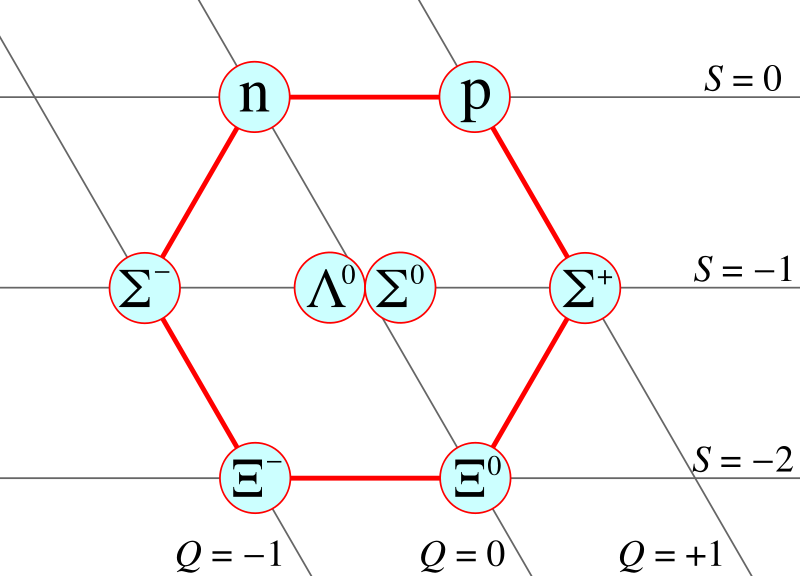
\includegraphics[width=0.45\textwidth]{baryon}}
\caption{Mesons and Baryons}
\end{figure}
  \ech
\end{frame}
\begin{frame}\frametitle{\bch The Eightfold Way\ech}
  \bch
  于是,Gell-Mann和Ne'eman分别独立指出:八个自旋为零的介子和八个自旋为$1/2$的介子可以得到$SU(3)$的八维伴随表示,就是我们的(1,1)型张量。随后,Gell-Mann指出,有10种((3,0)型张量得到的表示)baryon resonances,最后一种是$\Omega^-$。
   \begin{figure}
\centering  
\subfigure{
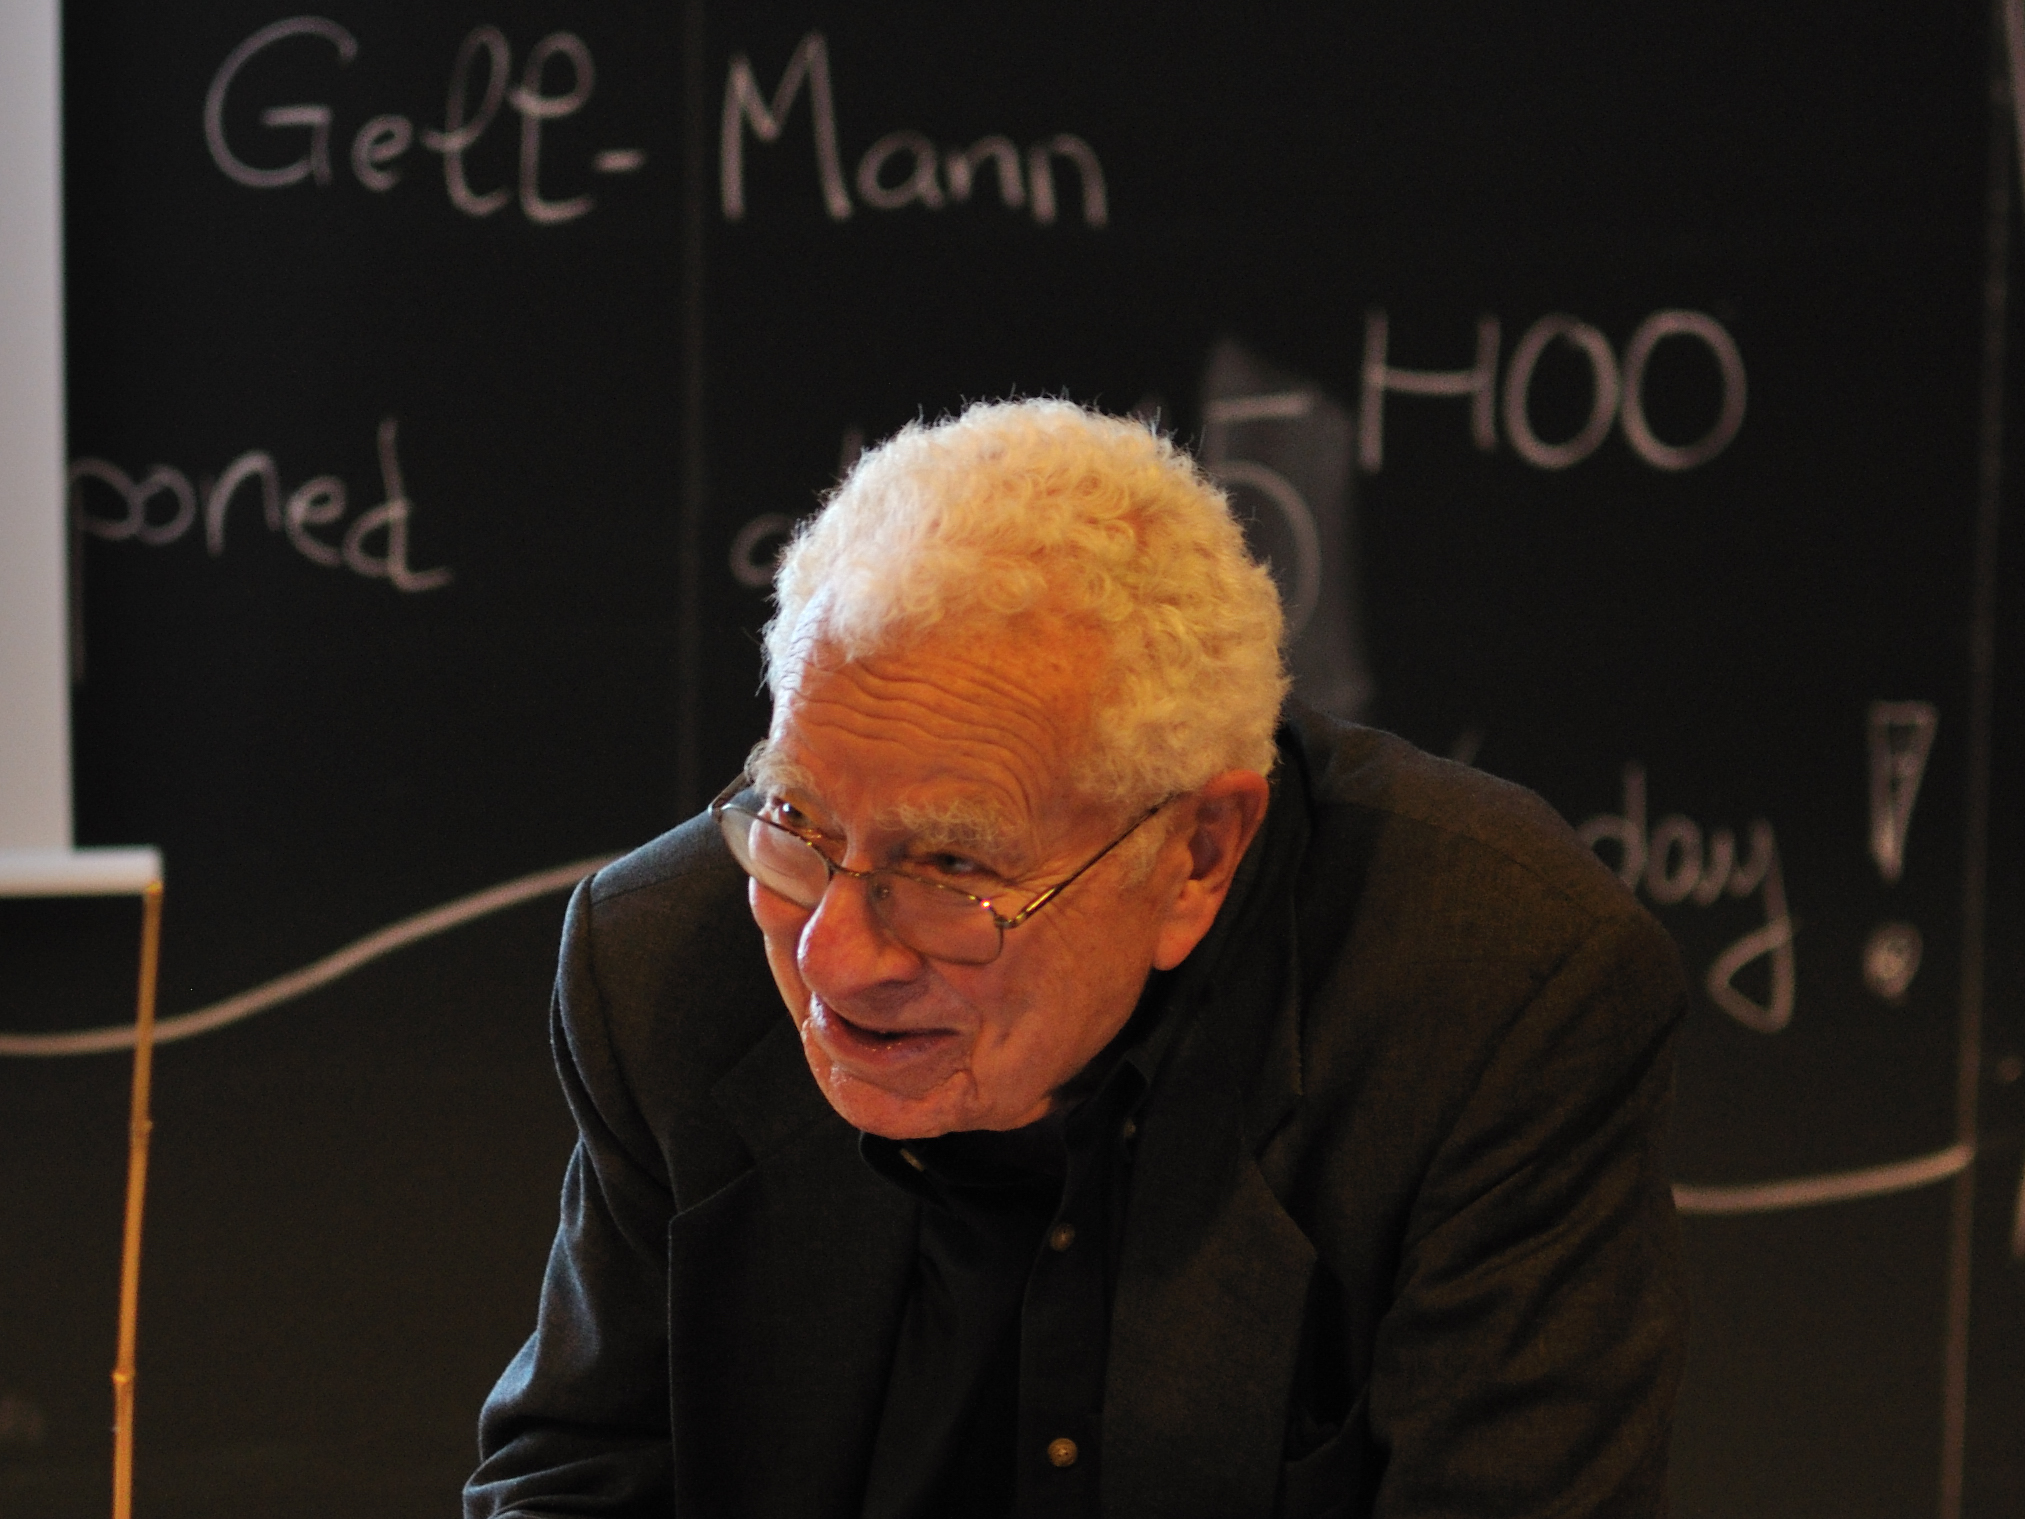
\includegraphics[scale=0.2]{gellmann}}
\subfigure{
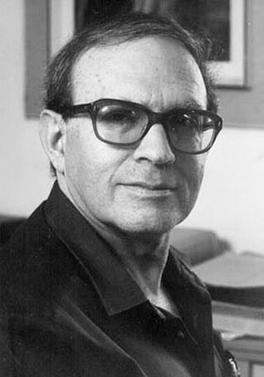
\includegraphics[scale=0.2]{neeman}}
\caption{Gell-Mann, Ne'eman}
\end{figure}
  \ech
\end{frame}
\begin{frame}\frametitle{Badly broken symmetry}
  \bch
  $SU(2)$的同位旋假说很成功,得到的粒子质量差不多,是一个近似对称性。但是$SU(3)$得到的质量就没有那么相近,我们可以忍受粒子质量差$20\% \sim 30\%$。重子的情况还好,但是$K$介子和$\pi$介子就差的离谱。
  \ech
\end{frame}
\begin{frame}\frametitle{\bch Quarks and Triality\ech}
  \bch
  上面的两个被实验观测到的对称性$(m,n)=(1,1)=8$和$(m,n)=(3,0)=10$不禁引发我们思考,因为他们都满足
  \be
  (m-n)\mod 3 =0 
  \ee
  我们把上面的这个余数叫做triality。可见,实验上只观测到了triality为0的粒子。
  \ech
\end{frame}
\begin{frame}\frametitle{\bch The center of a group\ech}
  \bch
  回想起我们定义过群的中心是和其他群元对易的群元的集合。我们之前讨论过$SU(N)$群的中心就是$Z_N$群。因此$SU(3)$群的中心是$\{I,z,z^2\}$,其中
  \be
  z\equiv
  \begin{pmatrix}
    e^{2\pi i/3} &0 & 0\\
    0&e^{2\pi i/3}&0 \\
    0&0&e^{2\pi i/3}
  \end{pmatrix}
  =e^{2\pi i/3}\begin{pmatrix}
    1&0&0\\
    0&1&0\\
    0&0&1
  \end{pmatrix}
  \ee
将这个群元作用在$(m,n)$型张量上,会使得$(m,n)$型张量多出相因子$e^{2\pi i(m-n)/3}$,这就是为什么triality出现的原因。
\ech
\end{frame}
\begin{frame}\frametitle{\bch Quark\ech}
  \bch
  实验只观测到了$(m-n)\mod 3=0$的粒子,给了强相互作用理论很大的暗示。这时候,你一定会问:“Where is the fundamental representation 3?”,这就是 Gell-Mann 当年在哥伦比亚大学中午吃饭的时候问的问题。 

  Gell-Mann 不久之后就搞出了构建$3$的粒子,上夸克$u$、下夸克$d$、奇异夸克$s$。$3^{*}$由反夸克$\bar{u},\bar{d},\bar{s}$构建。说的详细点,$(1,0)$对应于夸克,$(0,1)$对应于反夸克,所以很容易有
  \be
  \mathrm{triality} = (\mathrm{quark} - \mathrm{antiquark})\mod 3
  \ee
  \ech
\end{frame}
\begin{frame}\frametitle{Etymology}
  – Three quarks for Muster Mark!
  
  Sure he hasn't got much of a bark

  And sure any he has it's all beside the mark.
\end{frame}
\begin{frame}\frametitle{\bch 解释发现的重子和介子\ech}
  \bch
  有了基础表示对应的粒子,群论立刻就解释了发现的粒子。因为有
  \be
  3\otimes 3^{*} =8\oplus 1
  \ee
  所以介子是由一个夸克(对应于$3$)和反夸克(对应于$3^{*}$)构成的。又因为有
  \be
  3\otimes 3\otimes 3 = 10\oplus 8 \oplus 8\oplus 1
  \ee
  所以重子是三个夸克的束缚态。例如,质子为uud,中子为udd,等等。同理,这个$10$种baryon resonance 也应该是三个夸克束缚在一起,我们惊奇的发现,$\Omega^-$是sss构成的。
  \ech
\end{frame}
\section{Decomposition}
\secpage{从$SU(3)$回到$SU(2)$}{$3\rightarrow 2_1 \oplus 1_{-2}$}
\begin{frame}\frametitle{\bch 从$SU(3)$回到$SU(2)$\ech}
  \bch
  我们现在试图从$SU(3)$回到海森堡的$SU(2)$同位旋理论。考虑$(1,0)$型张量$\psi^i$,很自然地拆分成$\psi^i=\{\psi^a,\psi^3\}$,其中$a$从1取到2。

  这意味着只变换$\psi$的前两个分量,而始终保持第三个分量不变。我们知道前两个分量是
  上夸克和下夸克,也就是说可以将前两个分量变换成上夸克和下夸克的线性组合。当上下夸克互相变换的时候,正好是质子和中子的互相变换。因此如果保持第三个奇异夸克分量不变,我们成功将$SU(3)$拆成原来的,即
  \be
  3 \rightarrow 2\oplus 1
  \ee
  \ech
\end{frame}

\begin{frame}\frametitle{更细致的拆分\ech}
  \bch
  刚刚我们拆分的方法简单粗暴,如果考虑的更多一点,得到$SU(3)$最大的子群:$SU(3)\rightarrow SU(2)\oplus U(1)$,这里$U(1)$中的元素是$e^{i\theta Y}$,其中
  \be
  Y=\frac{1}{3}
  \begin{pmatrix}
    1&0&0\\
    0&1&0\\
    0&0&-2
  \end{pmatrix}
  \ee
  其中$Y$又被称作超电荷矩阵。观察$Y$,它是个无迹厄米矩阵,而且变换时候不会改变前两个分量,故确实可以做这种分解,这种分解记为
  \be
  3\rightarrow (2,1)\oplus (1,-2)
  \ee
  其中括号的第一个数表示同位旋的维数,第二个数就是$3Y$,也可以写成更加紧凑的形式
  \be
  3\rightarrow 2_1 \oplus 1_{-2}
  \ee
  \ech
\end{frame}
\begin{frame}\frametitle{\bch 拆分$SU(3)$的所有表示\ech}
  \bch
  将上面的式子每一项都取厄米共轭,因为$SU(2)$怎么取共轭都不变,所以上面的拆分就变为
  \be
  3^{*}\rightarrow 2_{-1}+1_{2}
  \ee
  因为所有的表示都是由基础表示构建的,所以任何一个表示都可以按照上面两条式子拆分。
  \ech
\end{frame}
\begin{frame}\frametitle{\bch 给我们的粒子配对\ech}
  \bch
  考虑$3\otimes 3^{*}=8\oplus 1$,将等式左边用上面两个公式换掉,得到
  \be
  8\rightarrow 3\oplus 1\oplus 2\oplus 2
  \ee
  这说明八个介子或者重子由一个同位旋triplet,两个同位旋doublets,一个同位旋singlet构成,实验发现,果真如此。
  \begin{table}[H]
    \centering
    \begin{tabular}{|c|c|c|}
      \hline
      &介子&重子\\
      \hline
        isospin triplet &$\pi^+,\pi^0,\pi^-$& $\Sigma^+,\Sigma^0,\Sigma^-$\\
        isospin doublets & $K^+,K^0;\bar{K}^0,K^-$ & $\Xi^0,\Xi^-;n,p$\\
        isospin singlet &$\eta$ & $\Lambda$\\
        \hline
        
      \end{tabular}
    \end{table}
  \ech
\end{frame}
\begin{frame}\frametitle{\bch 使用更细致的分解\ech}
  \bch
  利用$SU(3)\rightarrow SU(2)\oplus U(1)$,可以得到(注意数$Y$在相乘的过程中只是相加,因为是简单的$U(1)$群)
  \be
  8\rightarrow 3_0\oplus 1_0\oplus 2_{3}\oplus 2_{-3}
  \ee
  这意味着对于triplet 和singlet,$Y=0$,对于doublets:$Y =\pm 1$
  \ech
\end{frame}
\begin{frame}\frametitle{\bch 等价方法:拆分张量\ech}
  \bch
  将张量拆成低维的张量也可以等效的得到上面的拆分,例如对于上面的$3\otimes 3^{*}$,便可以这样拆分
  \be
  \varphi^i_j = \{\bar{\varphi}^a_b,\varphi^a_3,\varphi^3_a,\varphi^3_3\}
  \ee
  其中的bar表示那是个无迹张量。
  \ech
\end{frame}
\begin{frame}\frametitle{\bch 电荷\ech}
  \bch
  在上一节中,我们曾经启发性的推导了$Q = I + \frac{1}{2}Y$,我们曾经说,$Y$是在$SU(2)$之外的一个算符,当时我们对于$Y$的值无能为力。但是现在,可以看到,对于doublets,$Y=1$,所以电荷为$Q = (1,0)$,对于triplet,电荷为$Q = (1,0,-1)$。但是如果将这个规则运用到夸克上,就出现了奇妙的事情,因为$3\rightarrow 2_1\oplus 1_{-2}$,那么得到$Q = (\frac{2}{3},-\frac{1}{3},-\frac{1}{3})$。可见夸克具有分数的电荷,在早期寻找夸克的努力中,就是冲着分数电荷去的。
  \ech
\end{frame}
\begin{frame}\frametitle{\bch 未完待续\ech}
  \bch
  我们对于$SU(3)$和粒子物理还有很多的话要讲,但是在那之前,我们需要仔细学习$SU(3)$代数。所以我们今天的故事就到这里结束了。
  \cpic{0.2}{continue}
  \ech
\end{frame}

\end{document}
